\documentclass{article}

\usepackage[paperheight=16.5cm,paperwidth=11.9cm]{geometry}
\pagenumbering{gobble}

\usepackage[pdfstartview=Fit]{hyperref}

\usepackage{animate}
\usepackage{media9}
\usepackage{tikz}
\usepackage{ifthen}
\usepackage{xcolor}

\usepackage[absolute,overlay]{textpos}

\DeclareSymbolFont{extraup}{U}{zavm}{m}{n}
\DeclareMathSymbol{\varheart}{\mathalpha}{extraup}{86}
\DeclareMathSymbol{\vardiamond}{\mathalpha}{extraup}{87}

% Actually draw the card
% This will be called from within a tikz environment within a appropriatley
% shifted scope. Draw the card in the rectangle between (0,0) and (1,-1.4).
% Arguments:
%     #1 suit (clubs: 0, diamond: 1, heart: 2, spade: 3)
%     #2 value (ace: 1, 2-10, jack: 11, queen: 12, king: 13)
%     #3 selected (0 or 1)
% Keep this short, as it will be called thousands of times
\definecolor{selectedcolor}{RGB}{173,255,189}
\newcommand*{\doDrawCard}[3]{
    \ifthenelse{#3=1}{
        \draw[rounded corners=5pt,fill=selectedcolor] (0,0) rectangle ++(1,-1.4);
    }{
        \draw[rounded corners=5pt,fill=white] (0,0) rectangle ++(1,-1.4);
    }
    %\draw (0,-0.7) -- ++(1,0);
    %\draw (0,0) rectangle ++(1,-1.4);
    \ifthenelse{#1=0 \or #1=3}{
        \node[text centered,text width=1cm,below] at (0.5,0) {\getValue{#2}~\getSuit{#1}};
        \node[text centered,text width=1cm,below,rotate=180] at (0.5,-1.4) {\getValue{#2}~\getSuit{#1}};
    }{
        \node[text centered,text width=1cm,below,red] at (0.5,0) {\getValue{#2}~\getSuit{#1}};
        \node[text centered,text width=1cm,below,red,rotate=180] at (0.5,-1.4) {\getValue{#2}~\getSuit{#1}};
    }
}

\newcommand*{\drawMode}[1]{
    \begin{tikzpicture}
        \path[draw, use as bounding box] (0,0) rectangle ++(1,-1);
        \ifthenelse{#1=0}{
            \node at (0.5,-0.5) {\getSuit{0}};
        }{
            \ifthenelse{#1=1}{
                \node at (0.5,-0.5) {\getSuit{0}\getSuit{1}};
            }{
                \node[text centered, text width=1cm] at (0.5,-0.5) {\getSuit{0}~\getSuit{1}\\\getSuit{2}~\getSuit{3}};
            }
        }
    \end{tikzpicture}
}

\newcommand*{\getSuit}[1]{%
    \ifthenelse{#1=0}{$\clubsuit$}{\ifthenelse{#1=1}{$\vardiamond$}{\ifthenelse{#1=2}{$\varheart$}{$\spadesuit$}}}%
}
\newcommand*{\getValue}[1]{%
    \ifthenelse{#1=1}{A}{\ifthenelse{#1=11}{J}{\ifthenelse{#1=12}{Q}{\ifthenelse{#1=13}{K}{#1}}}}%
}


\textblockorigin{1cm}{1.5cm}
\setlength{\TPHorizModule}{1.1cm}
\setlength{\TPVertModule}{1cm}

% helper function for drawing card
\newcommand*{\drawCard}[5]{ % column, index, suit, value
    \begin{tikzpicture}
        \path[use as bounding box] (0,2) rectangle (8.7,-10);
        \ifthenelse{#4=0}{}{
            \begin{scope}[shift={(#1*1.1,-#2*0.5)}]
                \doDrawCard{#3}{#4}{#5}
            \end{scope}
        }
    \end{tikzpicture}
}

% draw button area
\newcommand*{\drawColumnButton}{
    \begin{tikzpicture}
        \path[use as bounding box] (0,0) rectangle (0.88,-10);
    \end{tikzpicture}
}
\newcommand*{\drawCardButton}{
    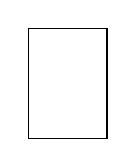
\begin{tikzpicture}
        \path[draw] (0,0) rectangle ++(1,-1.4);
    \end{tikzpicture}
}
\newcommand*{\drawGameButton}[1]{
    \begin{tikzpicture}
        \path[draw,use as bounding box] (0,0) rectangle ++(2,-1);
        \node at (1,-0.5) {#1};
    \end{tikzpicture}
}

% helper function to create animate object for a card
\newcommand*{\doMakeCard}[3]{ % column, index, label
    \begin{textblock}{2}[0,0](0,0)
        \begin{animateinline}[label=#3,nomouse]{1}
            \drawCard{#1}{#2}{0}{0}{0} \newframe
            %
            \drawCard{#1}{#2}{0}{1}{0} \newframe
            \drawCard{#1}{#2}{0}{2}{0} \newframe
            \drawCard{#1}{#2}{0}{3}{0} \newframe
            \drawCard{#1}{#2}{0}{4}{0} \newframe
            \drawCard{#1}{#2}{0}{5}{0} \newframe
            \drawCard{#1}{#2}{0}{6}{0} \newframe
            \drawCard{#1}{#2}{0}{7}{0} \newframe
            \drawCard{#1}{#2}{0}{8}{0} \newframe
            \drawCard{#1}{#2}{0}{9}{0} \newframe
            \drawCard{#1}{#2}{0}{10}{0} \newframe
            \drawCard{#1}{#2}{0}{11}{0} \newframe
            \drawCard{#1}{#2}{0}{12}{0} \newframe
            \drawCard{#1}{#2}{0}{13}{0} \newframe
            %
            \drawCard{#1}{#2}{1}{1}{0} \newframe
            \drawCard{#1}{#2}{1}{2}{0} \newframe
            \drawCard{#1}{#2}{1}{3}{0} \newframe
            \drawCard{#1}{#2}{1}{4}{0} \newframe
            \drawCard{#1}{#2}{1}{5}{0} \newframe
            \drawCard{#1}{#2}{1}{6}{0} \newframe
            \drawCard{#1}{#2}{1}{7}{0} \newframe
            \drawCard{#1}{#2}{1}{8}{0} \newframe
            \drawCard{#1}{#2}{1}{9}{0} \newframe
            \drawCard{#1}{#2}{1}{10}{0} \newframe
            \drawCard{#1}{#2}{1}{11}{0} \newframe
            \drawCard{#1}{#2}{1}{12}{0} \newframe
            \drawCard{#1}{#2}{1}{13}{0} \newframe
            %
            \drawCard{#1}{#2}{2}{1}{0} \newframe
            \drawCard{#1}{#2}{2}{2}{0} \newframe
            \drawCard{#1}{#2}{2}{3}{0} \newframe
            \drawCard{#1}{#2}{2}{4}{0} \newframe
            \drawCard{#1}{#2}{2}{5}{0} \newframe
            \drawCard{#1}{#2}{2}{6}{0} \newframe
            \drawCard{#1}{#2}{2}{7}{0} \newframe
            \drawCard{#1}{#2}{2}{8}{0} \newframe
            \drawCard{#1}{#2}{2}{9}{0} \newframe
            \drawCard{#1}{#2}{2}{10}{0} \newframe
            \drawCard{#1}{#2}{2}{11}{0} \newframe
            \drawCard{#1}{#2}{2}{12}{0} \newframe
            \drawCard{#1}{#2}{2}{13}{0} \newframe
            %
            \drawCard{#1}{#2}{3}{1}{0} \newframe
            \drawCard{#1}{#2}{3}{2}{0} \newframe
            \drawCard{#1}{#2}{3}{3}{0} \newframe
            \drawCard{#1}{#2}{3}{4}{0} \newframe
            \drawCard{#1}{#2}{3}{5}{0} \newframe
            \drawCard{#1}{#2}{3}{6}{0} \newframe
            \drawCard{#1}{#2}{3}{7}{0} \newframe
            \drawCard{#1}{#2}{3}{8}{0} \newframe
            \drawCard{#1}{#2}{3}{9}{0} \newframe
            \drawCard{#1}{#2}{3}{10}{0} \newframe
            \drawCard{#1}{#2}{3}{11}{0} \newframe
            \drawCard{#1}{#2}{3}{12}{0} \newframe
            \drawCard{#1}{#2}{3}{13}{0} \newframe
            %
            \drawCard{#1}{#2}{0}{1}{1} \newframe
            \drawCard{#1}{#2}{0}{2}{1} \newframe
            \drawCard{#1}{#2}{0}{3}{1} \newframe
            \drawCard{#1}{#2}{0}{4}{1} \newframe
            \drawCard{#1}{#2}{0}{5}{1} \newframe
            \drawCard{#1}{#2}{0}{6}{1} \newframe
            \drawCard{#1}{#2}{0}{7}{1} \newframe
            \drawCard{#1}{#2}{0}{8}{1} \newframe
            \drawCard{#1}{#2}{0}{9}{1} \newframe
            \drawCard{#1}{#2}{0}{10}{1} \newframe
            \drawCard{#1}{#2}{0}{11}{1} \newframe
            \drawCard{#1}{#2}{0}{12}{1} \newframe
            \drawCard{#1}{#2}{0}{13}{1} \newframe
            %
            \drawCard{#1}{#2}{1}{1}{1} \newframe
            \drawCard{#1}{#2}{1}{2}{1} \newframe
            \drawCard{#1}{#2}{1}{3}{1} \newframe
            \drawCard{#1}{#2}{1}{4}{1} \newframe
            \drawCard{#1}{#2}{1}{5}{1} \newframe
            \drawCard{#1}{#2}{1}{6}{1} \newframe
            \drawCard{#1}{#2}{1}{7}{1} \newframe
            \drawCard{#1}{#2}{1}{8}{1} \newframe
            \drawCard{#1}{#2}{1}{9}{1} \newframe
            \drawCard{#1}{#2}{1}{10}{1} \newframe
            \drawCard{#1}{#2}{1}{11}{1} \newframe
            \drawCard{#1}{#2}{1}{12}{1} \newframe
            \drawCard{#1}{#2}{1}{13}{1} \newframe
            %
            \drawCard{#1}{#2}{2}{1}{1} \newframe
            \drawCard{#1}{#2}{2}{2}{1} \newframe
            \drawCard{#1}{#2}{2}{3}{1} \newframe
            \drawCard{#1}{#2}{2}{4}{1} \newframe
            \drawCard{#1}{#2}{2}{5}{1} \newframe
            \drawCard{#1}{#2}{2}{6}{1} \newframe
            \drawCard{#1}{#2}{2}{7}{1} \newframe
            \drawCard{#1}{#2}{2}{8}{1} \newframe
            \drawCard{#1}{#2}{2}{9}{1} \newframe
            \drawCard{#1}{#2}{2}{10}{1} \newframe
            \drawCard{#1}{#2}{2}{11}{1} \newframe
            \drawCard{#1}{#2}{2}{12}{1} \newframe
            \drawCard{#1}{#2}{2}{13}{1} \newframe
            %
            \drawCard{#1}{#2}{3}{1}{1} \newframe
            \drawCard{#1}{#2}{3}{2}{1} \newframe
            \drawCard{#1}{#2}{3}{3}{1} \newframe
            \drawCard{#1}{#2}{3}{4}{1} \newframe
            \drawCard{#1}{#2}{3}{5}{1} \newframe
            \drawCard{#1}{#2}{3}{6}{1} \newframe
            \drawCard{#1}{#2}{3}{7}{1} \newframe
            \drawCard{#1}{#2}{3}{8}{1} \newframe
            \drawCard{#1}{#2}{3}{9}{1} \newframe
            \drawCard{#1}{#2}{3}{10}{1} \newframe
            \drawCard{#1}{#2}{3}{11}{1} \newframe
            \drawCard{#1}{#2}{3}{12}{1} \newframe
            \drawCard{#1}{#2}{3}{13}{1}
        \end{animateinline}
    \end{textblock}
}

% create regular card a position
\newcommand*{\makeCard}[2]{         % column, index
    \doMakeCard{#1}{#2}{c#1x#2}
}

% create card with custom label and action
\newcommand*{\makeSpecialCard}[3]{  % column, index, label
    \doMakeCard{#1}{#2/0.5}{#3}
}

\newcommand*{\makeButton}[1]{   % column
    \begin{textblock}{2}(#1,2)
        \mediabutton[jsaction={
            if(typeof(column_clicked) != "undefined")
                column_clicked(#1);
        }]{%
            \hspace*{-0.12cm}%
            \drawColumnButton
        }
    \end{textblock}
}

\newcommand*{\makeCardButton}[3]{   % column, index, action
    \begin{textblock}{2}(#1,0)
        \mediabutton[jsaction={
            if(typeof(special_clicked) != "undefined")
                special_clicked("#3");
        }]{%
            \hspace*{-0.12cm}%
            \drawCardButton
        }
    \end{textblock}
}

\newcommand*{\makeGameButton}[4]{   % column, index, text, action
    \begin{textblock}{2}(#1,#2)
        \mediabutton[jsaction={
            #4
        }]{%
            \hspace*{-0.12cm}%
            \drawGameButton{#3}
        }
    \end{textblock}
}

\newcommand*{\drawBackground}{
    \definecolor{tablecolor}{RGB}{62, 114, 17}
    \begin{textblock}{2}[0,0](-1,-1)
        \begin{tikzpicture}
            \path[use as bounding box,draw,fill=tablecolor] (0,2) rectangle (10.9,-12);
        \end{tikzpicture}
    \end{textblock}
}


\pgfmathsetmacro\numCols{8}
\pgfmathsetmacro\maxStack{16}

\begin{document}

\drawBackground

\foreach \i in {0,...,\numCols-1}{
    \foreach \j in {0,...,\maxStack-1}{
        \makeCard{\i}{\j}
    }
}

\makeSpecialCard{0.00}{-2}{o1}
\makeSpecialCard{0.95}{-2}{o2}
\makeSpecialCard{1.90}{-2}{o3}
\makeSpecialCard{2.85}{-2}{o4}

\makeSpecialCard{4.15}{-2}{f1}
\makeSpecialCard{5.10}{-2}{f2}
\makeSpecialCard{6.05}{-2}{f3}
\makeSpecialCard{7.00}{-2}{f4}

\foreach \i in {0,...,\numCols-1}{
    \makeButton{\i}
}

\makeCardButton{0.00}{-2}{o1}
\makeCardButton{0.95}{-2}{o2}
\makeCardButton{1.90}{-2}{o3}
\makeCardButton{2.85}{-2}{o4}

\makeCardButton{4.15}{-2}{f1}
\makeCardButton{5.10}{-2}{f2}
\makeCardButton{6.05}{-2}{f3}
\makeCardButton{7.00}{-2}{f4}

\makeGameButton{2}{13.5}{Deal cards}{
    deck_size = 52;
    markedColumn = undefined;
    function get_card(col, idx) {return anim["c" + col + "x" + idx].frameNum - 1;}
    function set_card(col, idx, id) {anim["c" + col + "x" + idx].frameNum = 1 + id;}
    function set_card_s(label, id) {anim[label].frameNum = 1 + id;}
    function get_card_s(label) {return anim[label].frameNum - 1;}
    function shuffle(num_suits) {
        single_suit = num_suits == 1;
        num_cards = num_suits * 13;
        perm = [];
        for(i = 0; i < deck_size; i++)
            perm.push([Math.random(), i]);
        perm = perm.sort();
        for(idx = 0; idx < \maxStack; idx++) {
            for(col = 0; col < \numCols; col++) {
                if(idx*\numCols+col < deck_size)
                    set_card(col, idx, mod(perm[idx*\numCols+col][1], num_cards));
                else
                    set_card(col, idx, -1);
            }
        }
        set_card_s("o1", -1);
        set_card_s("o2", -1);
        set_card_s("o3", -1);
        set_card_s("o4", -1);
        set_card_s("f1", -1);
        set_card_s("f2", -1);
        set_card_s("f3", -1);
        set_card_s("f4", -1);
    }
    function get_column_length(col) {
        for(i = 0; i < \maxStack; i++)
            if(get_card(col, i) == -1)
                return i;
        return \maxStack;
    }
    function get_top_card(col) {
        len = get_column_length(col);
        if(len == 0) return -1;
        return get_card(col, len-1);
    }
    function get_num_marked(col) {
        for(i = 0; i < \maxStack; i++)
            if(get_card(col, i) >= deck_size)
                return i;
        return \maxStack;
    }
    function mod(x,y) {return x - Math.floor(x/y)*y;}
    function can_put_on_top(bottom, top) {
        if(bottom == -1) return true;
        if(mod(bottom,13) != mod(top + 1,13)) return false;
        if(mod(bottom,13) == 0) return false;
        if(single_suit) return true;
        s1 = Math.floor(bottom/13);
        s2 = Math.floor(top/13);
        if((s1 == 0) || (s1 == 3)) return (s2 == 1) || (s2 == 2);
        return (s2 == 0) || (s2 == 3);
    }
    function column_clicked(col) {
        if(typeof(markedColumn)=="undefined") {
            if(get_column_length(col) > 0) {
                markedColumn = col;
                set_card(col, get_column_length(col)-1, get_top_card(markedColumn) + deck_size);
                return;
            }
        } else if(markedColumn == col) {
            m = get_num_marked(col);
            if(m>0 && can_put_on_top(get_card(col, m-1), get_card(col, m) - deck_size))
                set_card(col, m-1, get_card(col, m-1) + deck_size);
            else {
                for(num = get_num_marked(col); num < get_column_length(col); num++)
                    set_card(col, num, get_card(col, num) - deck_size);
                markedColumn = undefined;        
            }
        } else if(markedColumn < 0) {
            label = "o" + (-markedColumn);
            if(get_column_length(col) < \maxStack && can_put_on_top(get_top_card(col), get_card_s(label) - deck_size)) {
                set_card(col, get_column_length(col), get_card_s(label) - deck_size);
                set_card_s(label, -1);
                markedColumn = undefined;
            }
        } else {
            num1 = get_num_marked(markedColumn);
            if(get_column_length(col) + get_column_length(markedColumn) - num1 > \maxStack)
                return;
            if(can_put_on_top(get_top_card(col), get_card(markedColumn, num1) - deck_size)) {
                top_card = get_column_length(markedColumn);
                for(num = num1; num < top_card; num++) {
                    set_card(col, get_column_length(col), get_card(markedColumn, num) - deck_size);
                    set_card(markedColumn, num, -1);
                }
                markedColumn = undefined;
            }
        }
    }
    function special_clicked(label) {
        if(typeof(markedColumn)=="undefined") {
            if(label.startsWith("o") && get_card_s(label) != -1) {
                set_card_s(label, get_card_s(label) + deck_size);
                markedColumn = -parseInt(label.slice(1));
            }
        } else if(markedColumn < 0) {
            if(label.startsWith("o")) {
                o = parseInt(label.slice(1));
                if(o == -markedColumn) { 
                    if(get_card_s(label) >= deck_size) {
                        set_card_s(label, get_card_s(label) - deck_size);
                        markedColumn = undefined;
                    }
                } else {
                    if(get_card_s(label) == -1) {
                        set_card_s(label, get_card_s("o" + (-markedColumn)) - deck_size);
                        set_card_s("o" + (-markedColumn), -1);
                        markedColumn = undefined;
                    }
                }
            } else {
                selected = get_card_s("o" + (-markedColumn));
                if((get_card_s(label) == -1 && mod(selected, 13) == 0) || (get_card_s(label) == selected - deck_size - 1)) {
                    set_card_s(label, selected - deck_size);
                    set_card_s("o" + (-markedColumn), -1);
                    markedColumn = undefined;
                    if(mod(get_card_s("f1"),13)==12 && mod(get_card_s("f2"),13)==12 && mod(get_card_s("f3"),13)==12 && mod(get_card_s("f4"),13)==12) {
                        set_card_s("f1", get_card_s("f1") + deck_size);
                        set_card_s("f2", get_card_s("f2") + deck_size);
                        set_card_s("f3", get_card_s("f3") + deck_size);
                        set_card_s("f4", get_card_s("f4") + deck_size);
                    }
                }
            }
            return
        } else if(get_num_marked(markedColumn) != get_column_length(markedColumn)-1)
            return;
        else if(label.startsWith("o")) {
            if(get_card_s(label) == -1) {
                set_card_s(label, get_top_card(markedColumn) - deck_size);
                set_card(markedColumn, get_column_length(markedColumn)-1, -1);
                markedColumn = undefined;
            }
        } else {
            selected = get_top_card(markedColumn);
            if((get_card_s(label) == -1 && mod(selected, 13) == 0) || (get_card_s(label) == selected - deck_size - 1)) {
                set_card_s(label, selected - deck_size);
                set_card(markedColumn, get_column_length(markedColumn)-1, -1);
                markedColumn = undefined;
                if(mod(get_card_s("f1"),13)==12 && mod(get_card_s("f2"),13)==12 && mod(get_card_s("f3"),13)==12 && mod(get_card_s("f4"),13)==12) {
                    set_card_s("f1", get_card_s("f1") + deck_size);
                    set_card_s("f2", get_card_s("f2") + deck_size);
                    set_card_s("f3", get_card_s("f3") + deck_size);
                    set_card_s("f4", get_card_s("f4") + deck_size);
                }
            }
        }
    }
    shuffle(Math.max(1, 2*anim["mode"].frameNum));
}

\begin{textblock}{2}(5,13.5)
    \begin{animateinline}[label=mode,poster=last,step]{1}
        \drawMode{0} \newframe
        \drawMode{1} \newframe
        \drawMode{2}
    \end{animateinline}
\end{textblock}

\end{document}
